\section{Vulnerabilities}
In the following sections will be explained the main vulnerabilities that EternalBlue uses to complete the remote code execution. 
Then, in the section Exploit (6.0) they will be liked together for the final overview of the attack.

\subsection{Integer cast error}
This vulnerability is due to an error in the computation of the allocation size of a buffer, it is considered the main bug because it is the one that creates the buffer overflow.\\
SMB gives the possibility to include in the headers of the message the File Extended Attributes (FEA) which is a data structure that 
associates files with metadata. Because there is the possibility to include more than one file, the FEAs are grouped up i na list structure called FEAList.
The following image shows how these two struct are composed.

\begin{figure}[ht!]
  \centering
    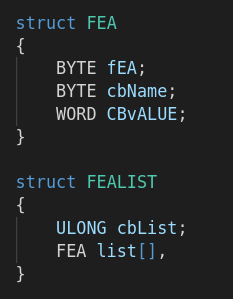
\includegraphics[scale=0.5]{images/FEA_code.png}
    \caption{FEA and FEAList structs}
\end{figure}
\noindent The FEAList struct has a variable called cbList used to memorize how many bytes is long the list of FEA.\\
Due to compatibility problems the FEAList that arrives to the Windows server in the header of the SMB message has to be casted to 
a custom list called NTFEAList, the following image shows how it is composed.

\begin{figure}[ht!]
  \centering
    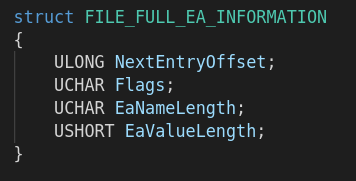
\includegraphics[scale=0.5]{images/windows_ea_struct.png}
    \caption{Windows NTFEAList}
\end{figure}
\noindent The two struct are quite different, so the server has to manage a cast function.\\
One of the first things that the cast function has to do is computing the size of the buffer that has to be allocated for the NTFEAList. To do that 
it looks to the value of cbList in the FEAList.
This function also checks that the value of cbList corresponds to the actual length of the FEAList, this is done by iterating over all the FEAs in the while cycle.
In case the value of cbList is not correct and it is more that what it is expected it changes the value of cbList with the real list size.\\
The following image shows the NTFEAList buffer size computation function.

\begin{figure}[ht!]
  \centering
    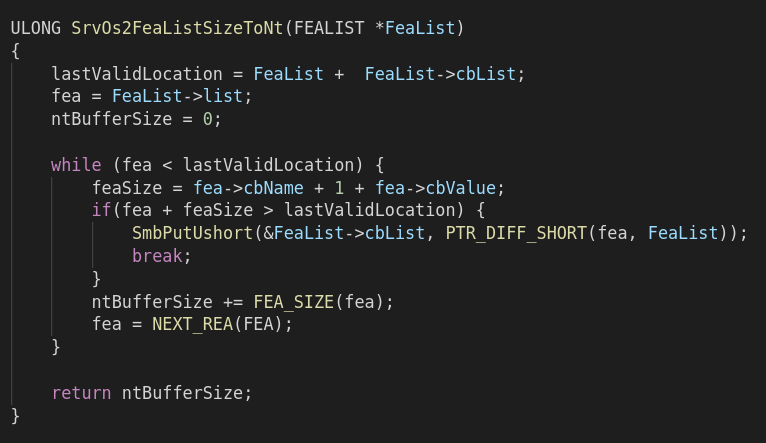
\includegraphics[scale=0.5]{images/SrvOs2FeaListSizeToNt.png}
    \caption{FEA to NT casting function}
\end{figure}

\noindent This size fixing operation is the vulnerability because it considers the cbList as a UShort type (16 bit), instead it is a ULong type (32bit).
Because of that it allocates less space then what the list needs causing an overflow of the NT buffer in the heap\cite{exploit-db}.
The following image shows clearly the incompatible types of cbList and the method SmbPutUshort().
\begin{figure}[ht!]
  \centering
    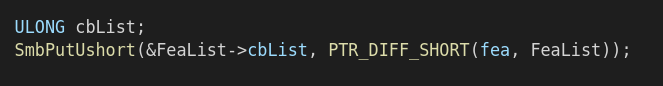
\includegraphics[scale=0.5]{images/vulnerable_lines.png}
    \caption{Integer cast error code}
\end{figure}

\clearpage

\subsection{Mixing transaction types}
Let's consider two different kinds of transaction in the SMB implementation:
\begin{itemize}
  \item SMB\_COM\_TRANSACTION2 and SMB\_COM\_TRANSACTION2\_SECONDARY: use WORD size parameters
  \item SMB\_COM\_NT\_TRANSACT and SMB\_COM\_NT\_TRANSACT\_SECONDARY: use DWORD size parameters
\end{itemize}
They are very similar but used for different scopes: the trans2 are used for managing FEAs, instead the NTtrans are used for the 
transfer of large blocks of data.
During the transmission of the FEAs we have to use the trans2 type, that is a problem for the attacker because this kind of transactions limit
the parameters size as a WORD, so he will not be able to trigger the main bug.
However there is a small bug that can help the attacker to work around this problem. The system doesn't check if the transactions types are 
consistent across the communication, so he can initialize the connection with an SMB\_COM\_NT\_TRANSACT which use DWORD parameters, and then continue with SMB\_COM\_TRANSACTION2\_SECONDARY.

\begin{figure}[ht!]
  \centering
    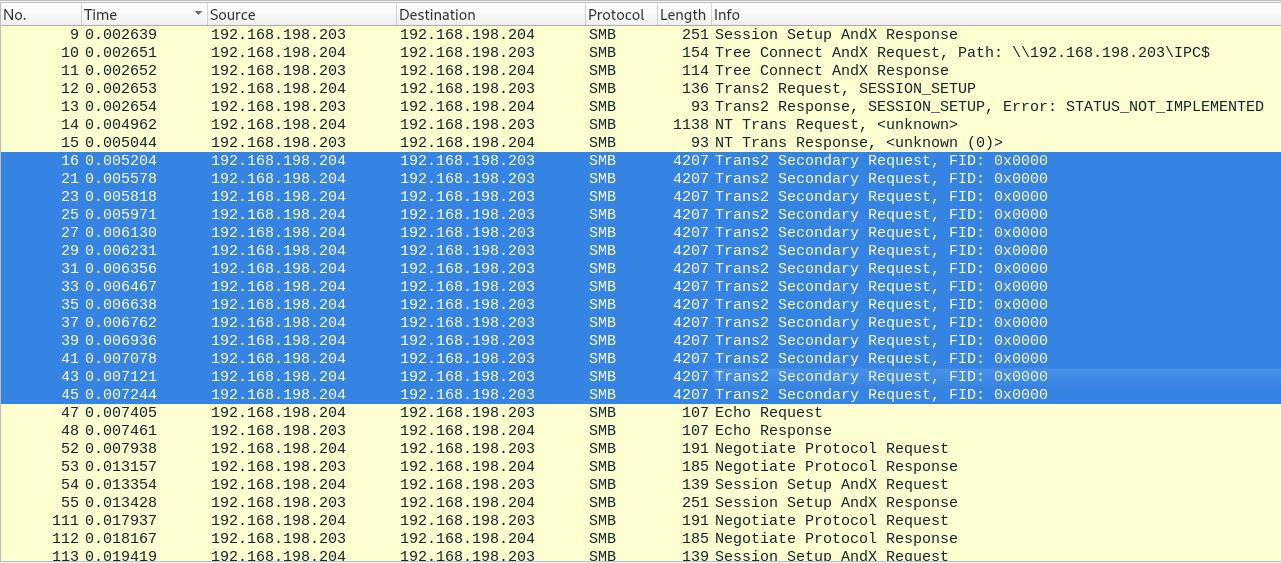
\includegraphics[scale=0.35]{images/ws_trans2_requests.png}
    \caption{Mixing transaction types}
\end{figure}

\clearpage

\subsection{Session setup allocation error}
In the implementation of SMB V1 there are two kinds of authentication:
\begin{itemize}
  \item LM/NTLM
  \item NTLMv2
\end{itemize}
The choice between is done at the beginning of the session setup with the command
SMB\_COM\_SESSION\_SETUP\_ANDX containing the parameters of LM/NTM or NTMv2.
The following images shows how these parameters and values are composed.


\begin{figure}[h]
    
  \begin{subfigure}{0.5\textwidth}
    \begin{center}
      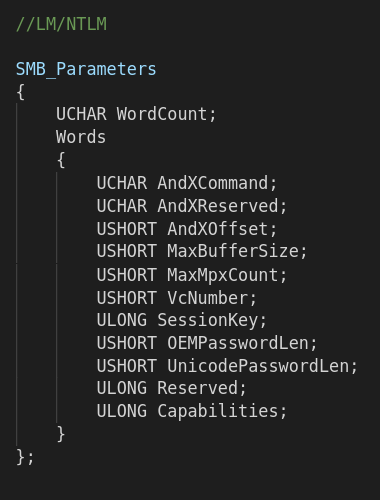
\includegraphics[scale=0.35]{images/lm_ntm_params.png}
    \end{center}
  \end{subfigure}
  \begin{subfigure}{0.5\textwidth}
    \begin{center}
      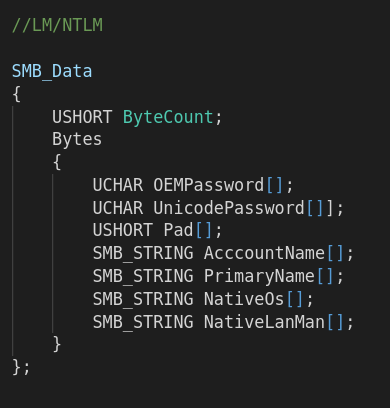
\includegraphics[scale=0.35]{images/lm_ntm_data.png}
    \end{center}
  \end{subfigure}
  \caption{LM/NTLM parameters and data}
\end{figure}



\begin{figure}[h]
    
  \begin{subfigure}{0.5\textwidth}
    \begin{center}
      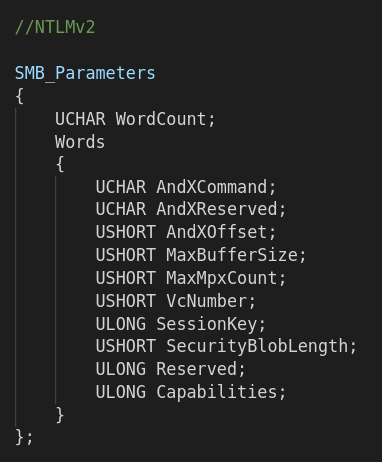
\includegraphics[scale=0.35]{images/ntlmv2_params.png}
    \end{center}
  \end{subfigure}
  \begin{subfigure}{0.5\textwidth}
    \begin{center}
      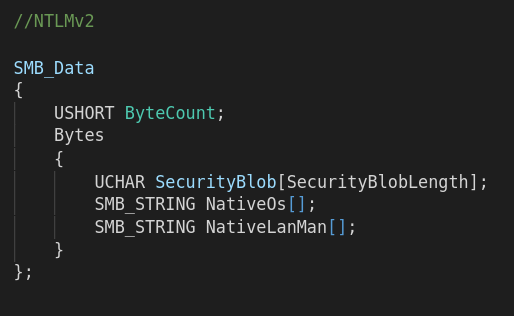
\includegraphics[scale=0.35]{images/ntlmv2_data.png}
    \end{center}
  \end{subfigure}
  \caption{NTLMv2 parameters and data}
\end{figure}

\noindent Notice that the ByteCount value indicates how much memory the server has to allocate for the session.\\
\noindent The choice between these two is done by checking 
if the wordCount is 13 (LM/NTLM) or 12 (NTLMv2), in this second case it looks also if it is defined the 
CAP\_EXTENDED\_SECURITY. If one of these conditions is not satisfied the request is rejected with an error.
The server after the first check controls again that it has CAP\_EXTENDED\_SECURITY and the
FLAGS\_EXTENDED\_SECURITY in the header, if this is true this is considered as NTLMv2 request.\\
\noindent Here there is the bug: the attacker can send a structure for NTLMv2 without setting the flag FLAGS\_EXTENDED\_SECURITY in the 
header. The server will interpret it as a LM/NTLM authentication when instead it is NTLMv2.\\
The following image shows the server side function for the detection of the authentication method.

\begin{figure}[ht!]
  \centering
    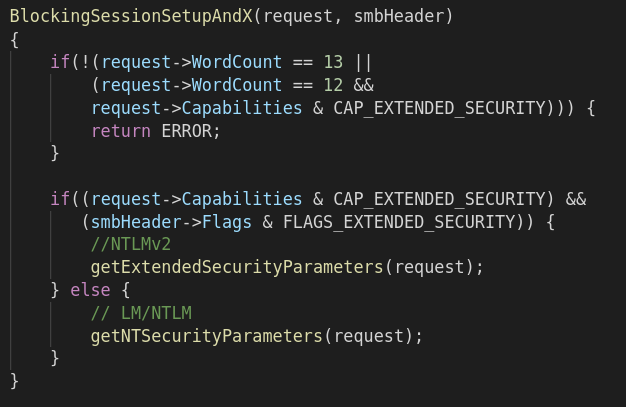
\includegraphics[scale=0.35]{images/auth_vuln_code.png}
    \caption{Session setup allocation error code}
\end{figure}

\noindent Now the server thinks that the words in the structure are 13 instead of 12. Because of that the server reads the ByteCount value inside the 
SMB\_STRING buffers, so the attacker is able to allocate how much memory he wants. \\
This is called remote heap allocation and it will be very useful to control in which part of the memory the NT buffer overflows.